\section{نتایج عملی}\label{sec:experiments}

در این پروژه ما ابزار
\lr{EStResT}
را پیاده‌سازی کرده و بهبود داده‌ایم.
به کمک این ابزار، می‌توانیم یک ساختمان رویداد تعریف کنیم،
آن را به یک مدل دودویی ترجمه کنیم
و مساله علت واقعی را روی مدل ترجمه شده بررسی کنیم.
تعریف مدل علّی دودویی و بررسی مساله علت واقعی 
روی این مدل نیز به تنهایی در این ابزار ممکن است.
با توجه به پیچیدگی پیدا کردن
$W$ و $w$
در حالت غیربهینه، حل مساله علیت در این ابزار
نیازمند ارائه این دو آرگومان نیز می‌باشد.

بهبودهای عملکرد این ابزار به طور کلی
در دو دسته قرار می‌گیرند:

\begin{enumerate}
  \item
    بهبود چندجمله‌ای عملکردهای موجود
    در نسخه اولیه ابزار
  \item
    بهبود روش حل مساله علیت
    به کمک تئوری‌های ارائه شده در بخش
    \ref{sec:improvements}
\end{enumerate}

در ادامه به بررسی هر کدام از این بخش‌ها می‌پردازیم.

\subsection{بهبود چندجمله‌ای عملکردهای موجود}

در ترخیص
\LTRfootnote{Release}
اولیه این ابزار،
هدف اصلی درستی عملکرد بوده و به همین دلیل،
دو عملکرد محاسبه مقدار متغیرها در مدل علّی
(متد \lr{\texttt{evaluate}})
و ثابت نگه داشتن مجموعه‌ای از متغیرها
(متد \lr{\texttt{intervene}})
با روش ساده‌تری اما پرهزینه‌تری پیاده‌سازی شده بودند.

\textbf{بهبود زمان اجرای متد
\lr{\texttt{intervene}}
}
در نسخه اولیه ابزار، متد
\lr{\texttt{intervene}}
که برای ثابت کردن مقدار چند متغیر استفاده می‌شود،
به صورت زیر پیاده‌سازی شده بود:

\begin{algorithm}
  \caption{پیاده‌سازی اولیه متد
  \lr{\texttt{intervene}}}
  \begin{latin}
  \begin{algorithmic}[1]
    \Require{$M(U,V,F),W,w$}
    \Ensure{$W \in V$}
    \State $\mu \gets M$
    \For{$W_i \in W$}
      \State $\mu \gets \Copy(\mu)$
      \State $F_{\mu,W_i} \gets w_i$
    \EndFor
    \State \Return $\mu$
  \end{algorithmic}
  \end{latin}
\end{algorithm}

در نسخه بهبود یافته،
به جای ساختن یک کپی به‌ازای هر متغیر،
تنها یک کپی ساخته می‌شود و سپس مقداردهی‌های ثابت
روی این کپی اعمال می‌شود:

\begin{algorithm}
  \caption{پیاده‌سازی بهبود یافته متد
  \lr{\texttt{intervene}}}
  \begin{latin}
  \begin{algorithmic}[1]
    \Require{$M(U,V,F),W,w$}
    \Ensure{$W \in V$}
    \State $\mu \gets M$
    \State $\mu \gets \Copy(\mu)$ \Comment{\lr{Only one copy}}
    \For{$W_i \in W$}
      \State $F_{\mu,W_i} \gets w_i$
    \EndFor
    \State \Return $\mu$
  \end{algorithmic}
  \end{latin}
\end{algorithm}

برای بهبود متد
\lr{\texttt{evaluate}}
از ویژگی بدون دور بودن مدل علّی بازگشتی استفاده می‌کنیم
(هالپرن و پرل در
\cite{halpern2001causes}
به این ویژگی اشاره کرده‌اند)؛
با توجه به این ویژگی، می‌توانیم ترتیبی روی متغیرها
تعریف کنیم، و سپس مقدار متغیرهای مدل را
با توجه به این ترتیب محاسبه کنیم.
برای تعریف این ترتیب از روش
\lr{Topological Sort}
که برای گراف‌های جهتدار بدون دور تعریف شده است، استفاده می‌کنیم.
استفاده از این روش در مدل‌های بزرگ
(با چندهزار متغیر)
زمان اجرای متد
\lr{\texttt{evaluate}}
را به صورت قابل توجهی کاهش می‌دهد.

در نسخه اولیه ابزار، متد
\lr{\texttt{evaluate}}
بدون استفاده از فرض بدون دور بودن
و به صورت ساده پیاده‌سازی شده بود:

\begin{algorithm}
  \caption{پیاده‌سازی اولیه متد
  \lr{\texttt{intervene}}}
  \begin{latin}
  \begin{algorithmic}[1]
    \Require{$M(U,V,F)$}
    \For{$1 \leq \texttt{iter} \leq |V|$}
      \For{$V_i \in V$}
        \State $V_i \gets F_{V_i}(\Par(V_i))$
      \EndFor
    \EndFor
  \end{algorithmic}
  \end{latin}
\end{algorithm}

در نسخه بهبود یافته، این متد با کمک الگوریتم
$\TopolSort$
و استفاده از رابطه
$\Par^{-1}$
(مجموعه فرزندان یک راس)
پیاده‌سازی شده است:

\begin{algorithm}
  \caption{پیاده‌سازی بهبود یافته متد
  \lr{\texttt{intervene}}}
  \begin{latin}
  \begin{algorithmic}[1]
    \Require{$M(U,V,F)$}
    \State $V_{\texttt{sorted}} \gets \TopolSort(V, \Par^{-1})$
    \For{$V_i \in V_{\texttt{sorted}}$}
      \State $V_i \gets F_{V_i}(\Par(V_i))$
    \EndFor
  \end{algorithmic}
  \end{latin}
\end{algorithm}

\subsection{بهبود روش حل مساله علیت}

در ترخیض اولیه این ابزار، مساله علیت با تعریف اولیه آن
و بدون بهینه‌سازی‌های ارائه شده پیاده‌سازی شده بود.
در نسخه فعلی، بهبودهای ارائه شده در این گزارش
در این ابزار پیاده‌سازی شده
و درستی عملکرد آن‌ها نیز به کمک آزمون‌های واحد و بنچمارک
\LTRfootnote{Benchmark}
موجود آزموده شده است.
در این ابزار از یک سناریوی شبکه نرم‌افزار محور
\LTRfootnote{Software-defined network}
به عنوان بنچمارک استفاده شده است
که در ادامه توضیح داده می‌شود:

\begin{figure}
  \centering
  \def\W{1.25}
  \def\H{1.25}
  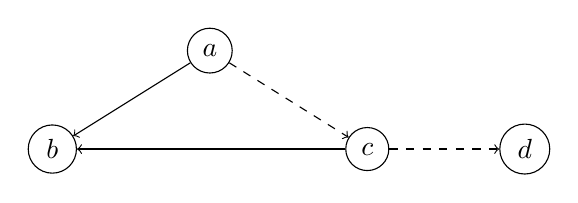
\begin{tikzpicture}
    \tikzset{
      host/.style={draw,circle}
    }
    \node[host] (a) at (0,\H) {$a$};
    \node[host] (b) at (-\W,0) {$b$};
    \node[host] (c) at (\W,0) {$c$};
    \node[host] (d) at (2*\W,0) {$d$};

    \path[->] (a) edge (b) edge[dashed] (c);
    \path[->] (c) edge (b) edge[dashed] (d);
  \end{tikzpicture}
  \caption{شبکه مثال لیست سیاه}
  \label{fig:blacklist-network}
\end{figure}

فرض کنیم شبکه‌ای با ۴ میزبان
$a$، $b$، $c$ و $d$
داریم و می‌خواهیم بسته‌ای از
$a$
را به صورت تصادفی در این شبکه
هدایت کنیم.
؛ این شبکه در شکل
\ref{fig:blacklist-network}
رسم شده است. در این شبکه،
$d$
در \textit{لیست سیاه}
\LTRfootnote{Blacklist}
$a$
قرار دارد، و هیچ‌گاه نباید مسیری از
$a$ به $d$
در این شبکه ساخته شود.
دو پردازه
$P$ و $Q$
دسترسی کنترل به این شبکه دارند و
می‌خواهند با ارسال دو پیام
$p$ و $q$،
به ترتیب یال‌های
$a \to b$ و $c \to b$
را با یال‌های
$a \to c$ و $c \to d$
جایگزین کنند.
واضح است که پس از ارسال این دو پیام
و نصب قوانین متناظر آن‌ها در شبکه،
مسیری از 
$a$ به $d$
تشکیل و ویژگی لیست سیاه در این شبکه نقض می‌شود.

برای این شبکه می‌توانیم ساختمان رویداد زیر را تعریف کنیم:

\begin{align*}
  E & = \set{p_1,q_1,ad_1,p_2,q_2,ad_2} \\ 
  \# & : p_1 \# q_2 \\
  \vdash & :
    \varnothing \vdash p_1,\,
    \varnothing \vdash q_2,\,
    \set{p_1} \vdash q_1,\,
    \set{q_2} \vdash p_2,\,
    \set{p_1,q_1} \vdash ad_1,\,
    \set{p_2,q_2} \vdash ad_2
\end{align*}

رویدادهای
$p_1$، $p_2$ و 
$q_1$، $q_2$
مربوط به دو ترتیب ممکن ارسال پیام‌های
$p$ و $q$
هستند. رویدادهای
$ad_1$ و $ad_2$
نیز برای نمایش وجود مسیر از
$a$ به $d$
در هر یک از ترتیب‌های ارسال تعریف شده‌اند.
شبکه پیکربندی‌های این ساختمان رویداد در شکل
\ref{fig:blacklist-configs}
آمده است. رفتار ناامن در این شبکه را به صورت زیر تعریف می‌کنیم:

\[ \varphi = \exists S
  \in \set{
    \set{p_1,q_1,ad_1},
    \set{q_2,p_2,ad_2}
  }.\;
  S \in \Conf(\ES)
\]

با توجه به این شبکه، به طور شهودی می‌توان
$p_1 \cancel{\#} q_1 (C_{p_1,q_1}=\bot)$
را به عنوان علتی برای رفتار ناامن در نظر گرفت.
صیحانی و دیگران در
\cite{seyhani2022}
نشان می‌دهند که با انتخاب
\[ W=C_{p_2,q_2},\,w=\top,\,\bar{x}=\top \]
مساله علیت برای رفتار ناامن مورد نظر را حل کنیم.

\begin{figure}
  \centering
  \def\W{2}
  \def\H{1.25}
  \begin{tikzpicture}
    \node (null)    at (0,0)      {$\varnothing$};
    \node (p1)      at (-\W,\H)   {$\set{p_1}$};
    \node (q2)      at (\W,\H)    {$\set{q_2}$};
    \node (p1q1)    at (-\W,2*\H) {$\set{p_1,q_1}$};
    \node (q2p2)    at (\W,2*\H)  {$\set{q_2,p_2}$};
    \node (p1q1ad1) at (-\W,3*\H) {$\set{p_1,q_1,ad_1}$};
    \node (q2p2ad2) at (\W,3*\H)   {$\set{q_2,p_2,ad_2}$};

    \path[->] (null) edge (p1) edge (q2);
    \path[->] (p1) edge (p1q1);
    \path[->] (q2) edge (q2p2);
    \path[->] (p1q1) edge (p1q1ad1);
    \path[->] (q2p2) edge (q2p2ad2);
  \end{tikzpicture}
  \caption{شبکه پیکربندی‌ها برای مثال لیست سیاه}
  \label{fig:blacklist-configs}
\end{figure}

در پیاده‌سازی عملی این شبکه، از ۱۲ رویداد استفاده شده است
(رویدادهایی که در این گزارش نیامده‌اند
برای مدل کردن یال‌های
$a \to b$ و $a \to c$
استفاده می‌شوند.)

در جدول
\ref{tab:blacklist-stats}
مقایسه‌ای بین
حالت اولیه و حالت بهبود یافته
برای این بنچمارک آمده است.
مقدارهای زمانی با واحد ثانیه نوشته شده‌اند.
برای مقدارهای زمانی، تایم‌اوت
\LTRfootnote{Timeout}
۶۰ ثانیه در نظر گرفته شده است.

\begin{table}
  \centering
  \begin{tabular}{ c|c|c|c|c }
    مرحله بهبود &
    $T_{\texttt{init}}+T_{\texttt{is\_cause}}$ &
    تعداد متغیرها &
    تعداد
    $Z$ها &
    $T_{\texttt{evaluate}}$ \\ \hline
    حالت اولیه (بدون بهبود) &
    $>60$ & 49218 & $2^{49216}$ & $>60$ \\ \hline
    بهینه‌سازی متد \lr{\texttt{evaluate}} &
    $>60$ & 49218 & $2^{49216}$ & $\mathbf{0.74}$ \\ \hline
    پیاده‌سازی تصویر $W$ &
    $>60$ & \textbf{546} & $2^{546}$ & $\mathbf{0.004}$ \\ \hline
    کاهش تعداد $Z$ها &
    $\mathbf{7.95}$ & 546 & \textbf{1} & $0.004$
  \end{tabular}
  \caption{جدول مقایسه برای بنچمارک لیست سیاه}
  \label{tab:blacklist-stats}
\end{table}
